\section{Levé topographique par pointage visuel sur une mire \label{CCS_MP_2017:p2}}
\begin{obj}
Montrer les limites en terme de facilité d'utilisation des mesures effectuées à l'aide d'un théodolite.
\end{obj}

La mesure par théodolite nécessite la présence de deux opérateurs:
\begin{itemize}
  \item un premier opérateur positionne le plus verticalement possible la mire (règle graduée) au point où la mesure topographique est à réaliser ;
  \item et un second opérateur pointe la ligne de visée vers la mire, met visuellement en coïncidence les traits de référence gravés sur le réticule, et situés à une distance $h$ l'un de l'autre, avec les points $A$ et $B$ de la mire (deux lentilles convexes permettent le rétablissement du sens d'origine de l'image) et finalement relève visuellement la différence de hauteur $H$ entre les points $A$ et $B$ (figure \ref{CCS_MP_2017:fig_03}).
  \end{itemize}

%Q 2. 
\question{\label{CCS_MP_2017:q_02}Déterminer la relation entre la distance focale de l'objectif $d$, la distance $h$ entre les deux traits de référence gravés sur le réticule, la distance $D$ à mesurer et la hauteur $H$ entre les points $A$ et $B$ sur la mire. Dans les appareils Leica, $d=100 \mathrm{~h}$ : calculer la valeur de la distance $D$ (en mètres) lorsque la hauteur $H=0,226 \mathrm{~m}$.}
\ifprof
\begin{corrige}
\end{corrige}
\else
\fi

La détermination de l'altitude d'un point permet de connaitre le dénivelé. Pour réaliser cette mesure, la hauteur d'instrument $L_{i}$ est d'abord mesurée précisément puis le bloc optique est pointé sur la même hauteur $L_{i}$ sur la mire : l'angle d'élévation $\theta_{i}$ est alors mesuré directement sur l'appareil (figure \ref{CCS_MP_2017:fig_04}).\\


%Q 3. 
\question{\label{CCS_MP_2017:q_03}Donner la relation entre le dénivelé $\delta$, la distance de mesure $D$ et l'angle d'élévation $\theta_{i}$. Pour une mesure $\theta_{i}=-4,723^{\circ}$ et pour la valeur de la distance $D$ obtenue question \ref{CCS_MP_2017:q_02} , donner la valeur du dénivelé $\delta$ (en mètres).}
\ifprof
\begin{corrige}
\end{corrige}
\else
\fi

\begin{figure}[!h]
\centering
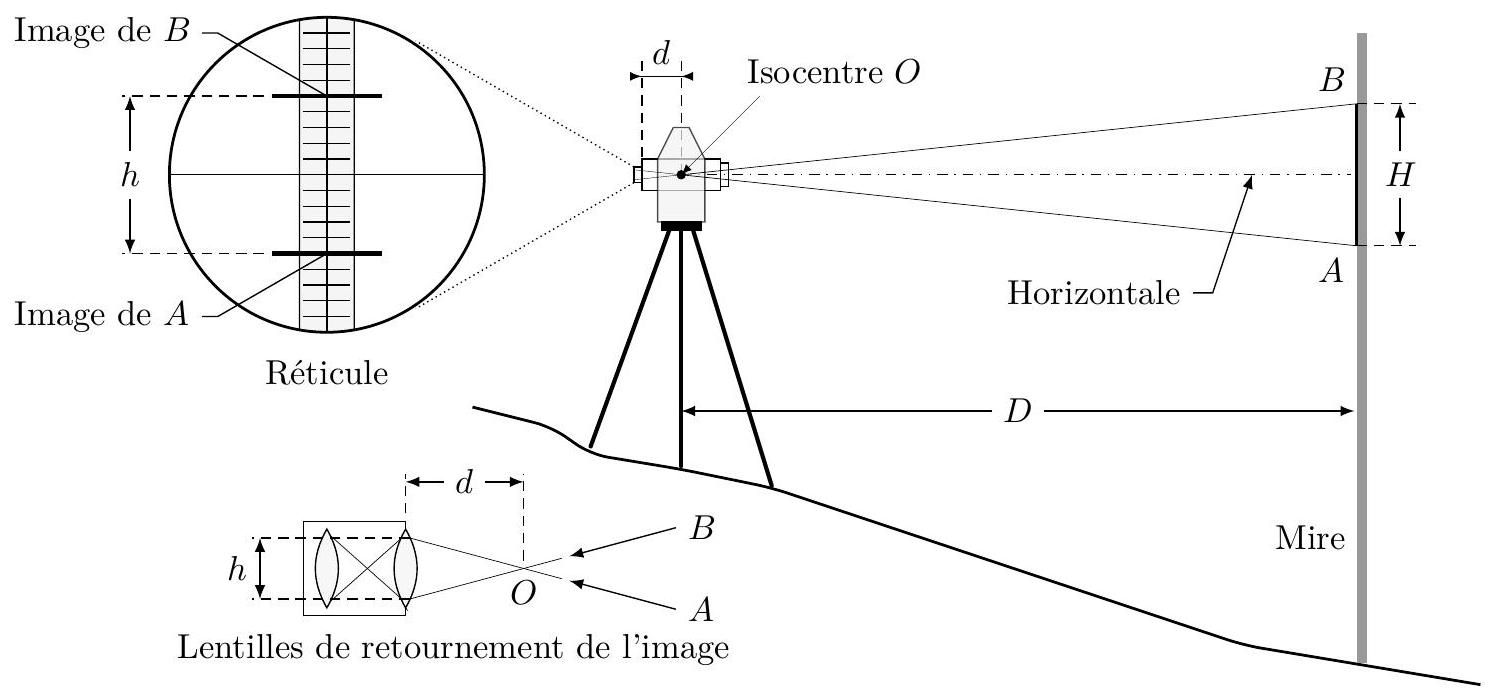
\includegraphics[width=\textwidth]{2024_12_07_51b7f57c7f055c2d8d29g-03(1)}
%Figure 3 
\caption{Mesure de la distance en utilisant un théodolite et une mire \label{CCS_MP_2017:fig_03}}
\end{figure}

\begin{figure}[!h]
\centering
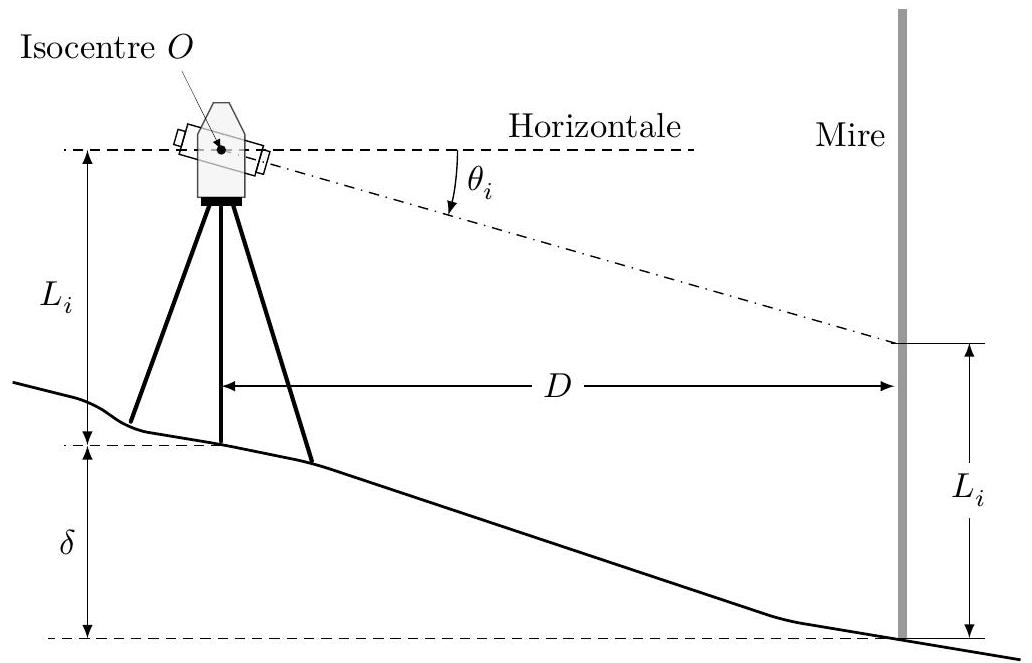
\includegraphics[width=.7\textwidth]{2024_12_07_51b7f57c7f055c2d8d29g-03}
%Figure 4 
\caption{Mesure du dénivelé en utilisant un théodolite et une mire \label{CCS_MP_2017:fig_04}}
\end{figure}

%Q 4. 
\question{\label{CCS_MP_2017:q_04}La distance $H$ est évaluée visuellement avec une incertitude $\Delta H=5 \mathrm{~mm}$ : déterminer la valeur de l'incertitude $\Delta D$ de la mesure de la distance $D$ (en mètres). La précision souhaitée pour la mesure de dénivelé de la question \ref{CCS_MP_2017:q_03}  étant de $0,01 \%$ (exigence du Bureau d'Études Topographiques Aérotopo pour que sa mesure soit valide selon les normes ISO), conclure sur la possibilité d'utiliser un théodolite, sachant que la résolution de la mesure angulaire en élévation est de $0,001^{\circ}$ sur les meilleurs appareils.}
\ifprof
\begin{corrige}
\end{corrige}
\else
\fi

Le levé topographique par théodolite est d'une précision liée à la qualité d'un relevé visuel : la qualité des mesures peut être grandement améliorée en utilisant un système de pointage laser sur un prisme optique rétroréfléchissant, ce qui est réalisé par le tachéomètre étudié dans la partie suivante.



